\section{Evaluation}

In this section, we evaluate \sys{} across three metrics: replication cost, replication time, and the optimizer solve time (or simply, runtime).
% 
In particular, we show that for intra-cloud and inter-cloud bulk data transfer, \sys{} is able to achieve up to 61.5\% cost improvements under a tight runtime budget when compared to academic, commercial, and open-source baselines.
% 
We also show that our approximations to reduce the optimizer solve time (as discussed in \cref{ss:approximations}) are highly effective by reducing the runtime by, on average, 30.68$\times$ for 5-destination replications. To simplify evaluation, we disable compression and encryption in experiments. 
%

%\subsection{Evaluated Systems and Algorithms} \label{sec:eval_baselines}
The full list of evaluated baselines is shown in \cref{tab:baselines}.
We note that many algorithms do not determine the number of VMs to use in each region.
To present them in the best light possible, we maximize the number of VMs in each region traversed by data, subject to per-region quota limits.



\if0
\begin{vitemize}
    \item \textbf{Direct}: Data is transferred directly from the source to the destination regions.  
    \item \textbf{MDST}: Data is transferred along edges selected by a Minimum Directed Spanning Tree (including source and destination regions) computed from network costs. 
    \item \textbf{Steiner Tree}: Data is transferred along edges selected by a Steiner tree (including optional waypoint regions) computed from network costs. 
    \item \textbf{SPIDER}~\cite{ganguly2005fast}: Data is transferred according to the plan generated by SPIDER, an academic baseline designed for fast bulk replication to multiple destinations.
    \item \textbf{CloudMPCast}~\cite{garcia2015cost}: Data is transferred along a set of cost-minimizing edges that meet a minimum bandwidth threshold. 
    %\item \textbf{Cost-aware Inter-DC Multicast}: Data is transferred according to a solver which models cost and deadlines in the inter-DC context (e.g. bandwidth and switch based pricing) as desribed by~\cite{fatemipour2022cost}. 
    \item \textbf{Deadline-aware Inter-DC Multicast}: Data is transferred to meet deadlines in the inter-DC context as described in~\cite{deadline2018}. 
    \item \textbf{AWS Multi-Region Bucket}~\cite{aws-replication}: Vendor product that supports intra-cloud between AWS regions only. We enable Replication Time Control~\cite{aws-replication-time-control}.
    \item \textbf{Bullet}~\cite{kostic2003bullet}: Data is transferred according to the plan generated by Bullet, a high bandwidth data dissemination technique using an overlay mesh.
    \item \textbf{BitTorrent}~\cite{twitter-bittorrent}: Peer-to-peer protocol where peers download data from each other in a decentralized manner.
    \item \textbf{Cloudcast-Opt (HT)}: Data is transferred along the highest throughput (HT) multicast tree generated by our optimizer given the tightest replication time constraint.
    \item \textbf{Cloudcast-Opt (LC)}: Data is transferred along the lowest cost (LC) multicast tree generated by our optimizer given a relatively loose replication time constraint.
\end{vitemize}
\fi

%Due to the large number of baseline algorithms and high cost of inter-cloud data transfer, we run comparisons across all academic baseline algorithms in simulation, and select the best performing baselines for end-to-end evaluation. 


% For transfers within a single cloud provider, we evaluate different academic baselines for generating multicast plans. 
% % 
% Each algorithm is implemented on top of \sys{}'s planner for consistency.
% % 
% We measure end-to-end replication time and the transfer cost.
% % 
% Many algorithms do not specify the number of VMs to use in each region, so we  maximize the number of VMs in each region which data traverses subject to per-region quota limits.
% % 
% % For example, if a waypoint region is selected by the Steiner tree, we create the maximum possible number of VMs in that region as our overlay routers.


\begin{figure}[t]
    \centering
    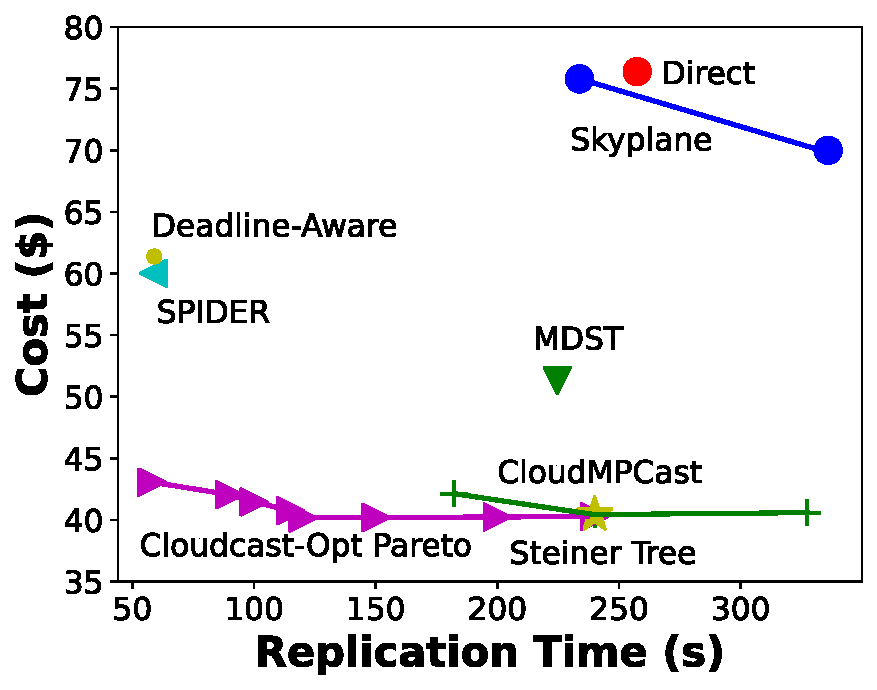
\includegraphics[width=
    0.35\textwidth]{figures/pareto.pdf}
    \caption{Simulated results for Multicast Algorithms.} 
    \label{fig:simulated-baselines}
\end{figure}

\begin{figure*}[tbp]
     \centering
     \begin{subfigure}[b]{0.33\textwidth}
        \centering
        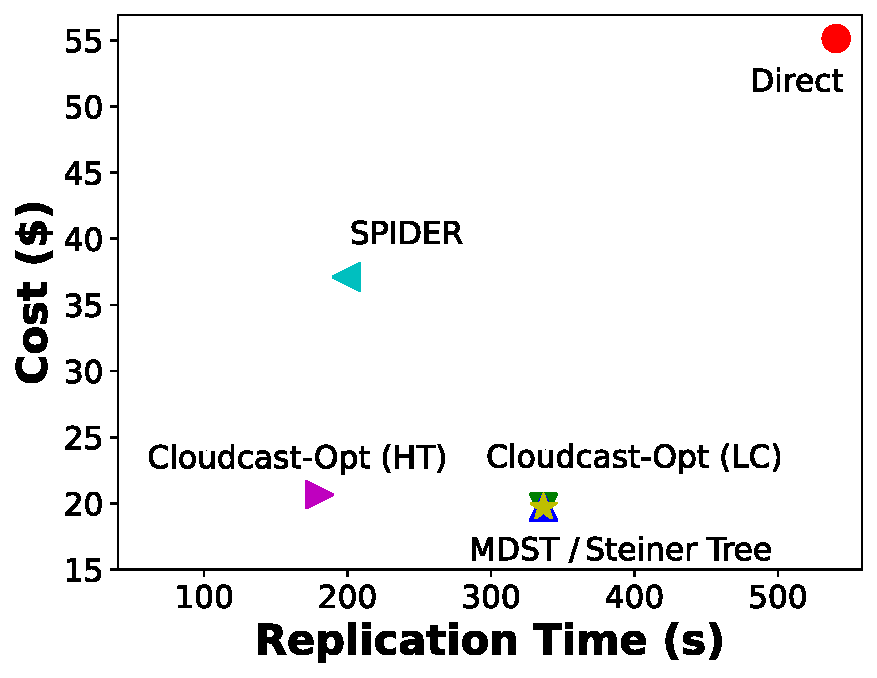
\includegraphics[width=\textwidth]{figures/aws.pdf}
        \caption{AWS Intra-Cloud}
        \label{fig:aws-intra-cloud}
    \end{subfigure}
    \hfill
    \begin{subfigure}[b]{0.33\textwidth}
        \centering
        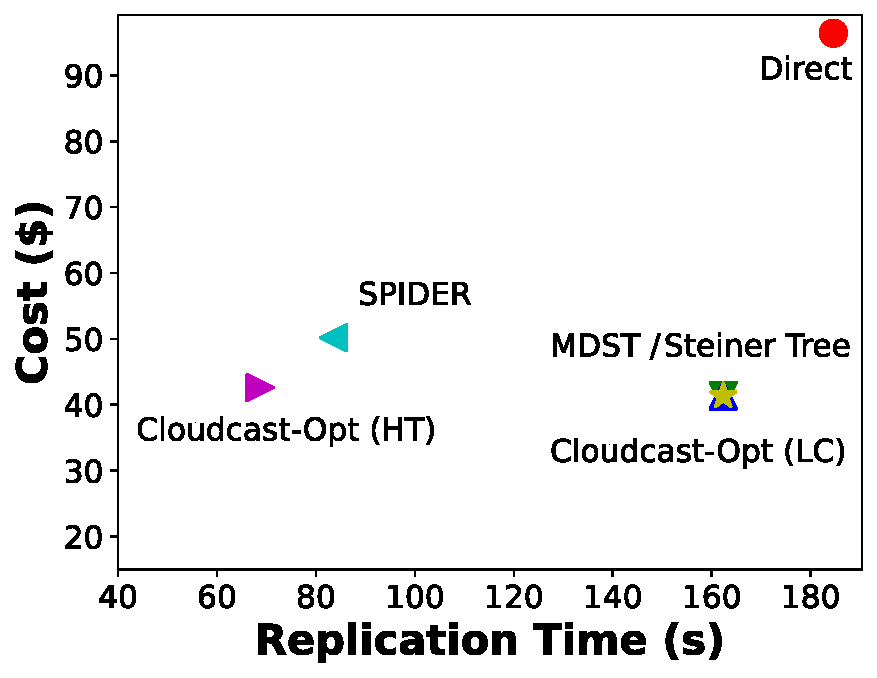
\includegraphics[width=\textwidth]{figures/azure.pdf}
        \caption{Azure Intra-Cloud}
        \label{fig:azure-intra-cloud}
    \end{subfigure}
    \hfill
    \begin{subfigure}[b]{0.33\textwidth}
        \centering
        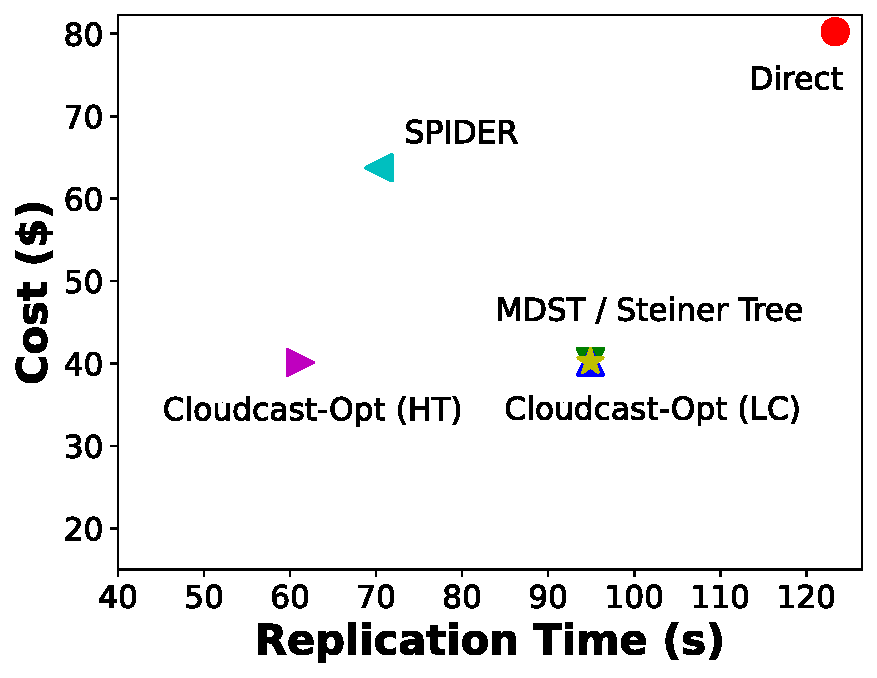
\includegraphics[width=\textwidth]{figures/gcp.pdf}
        \caption{GCP Intra-Cloud}
        \label{fig:gcp-intra-cloud}
    \end{subfigure}
    \hfill
    %\vspace{-2em}
    \caption{Intra-cloud multicast results for algorithms implemented on \sys{}.  
    %In all cases \sys{}-Opt is able to find significantly faster low-cost solutions where compared with existing techniques.  Furthermore, the MDST/Steiner Tree solution using ephemeral waypoints is able to consistently find the cost-optimal solution.  
    % \shu{we need to explain why we use these topologies, as well as why there are some variances in the running outcomes (e.g. SPIDER is closer to Cloudcast in Azure, or AWS runtime is much worse than the other cloud)}
    }
    \label{fig:intra-cloud}
\end{figure*}
\begin{figure}[tbp]
    \centering
    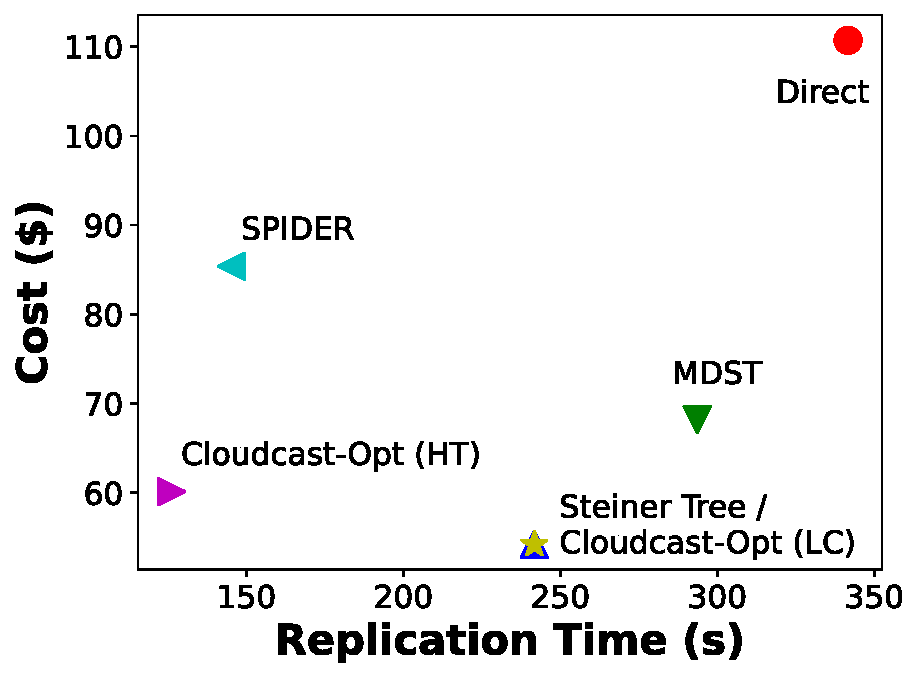
\includegraphics[width=
    0.33\textwidth]{figures/inter_cloud.pdf}
    \caption{Inter-cloud multicast results for different algorithms implemented on \sys{}. The \sys{} replication tree is visualized in Figure \ref{fig:example-topo}.
    % \joey{Figures should have a clear "takeaway" in the caption.  What would you say if presenting this figure in a talk.}
    }
    \label{fig:inter-cloud-1}
\end{figure}

\subsection{Comparison to Multicast Algorithms}
\label{sec:algorithm_eval}

% Using \sys{}, 
We compare the replication time and cost of existing multicast algorithms with \sys's optimizer to send 100\,GB of data from one source to six destination regions.

\heading{Simulation results}
Given the above replication scenario, we start by exploring a wide range of algorithmic baselines and \sys parameter settings through simulation.
While we tested many configurations through the development of \sys, due to limited space, we present results for a representative configuration\footnote{Simulated Inter-Cloud: from \path{gcp:asia-southeast1-a} to \path{azure:eastasia}, \path{aws:af-south-1}, \path{azure:brazilsouth}, \path{aws:sa-east-1}}.
Evaluated systems include \sys-Opt, direct transmission to the destinations, sending along cost-minimizing trees (MDST and Steiner Tree),  SPIDER~\cite{ganguly2005fast}, CloudMPCast~\cite{garcia2015cost}, Skyplane~\cite{jain2022skyplane}, and a deadline-aware inter-DC optimizer~\cite{deadline2018}.
Although Skyplane's optimizer is designed for unicast, not multicast, we adapt the optimizer's solution to multicast by running the optimization for each source-destination pair, and then combining all the graphs to build the distribution tree. 

For Skyplane, CloudMPCast, and \sys-Opt, we vary the throughput parameter to evaluate the performance range.  
For CloudMPCast~\cite{garcia2015cost}, the optimizer 
%it uses an optimizer that minimizes cloud egress costs by replicating data over min-cost Steiner Tree computed over edges with at least as much bandwidth as the the original source-destination path (to ensure minimal throughput degradation).
%CloudMPCast
allows for the level of throughput degradation to be controlled by an $\alpha \le 1$ term, which determines how aggressively edges are filtered out.
Our parameter sweep includes $\alpha \in [1, 0.5, 0.1]$, where $\alpha=1$ maximizes CloudMPCast's throughput.
For Skyplane, we vary the target throughput to maximize throughput and minimize cost, and plot both of these points. 
For \sys-Opt, we show results for several replication time constraints.

In \cref{fig:simulated-baselines}, we see that all baselines improve significantly upon direct transmission, and while some can match \sys-Opt's capacity for fast replication time or low cost, no existing baseline can optimize both metrics simultaneously.
Rather, \sys-Opt's Pareto-curve can match or beat all baselines on at least one of cost or performance.
CloudMPCast, whose $\alpha$ parameter does provide some flexibility, still offers a worse tradeoff than \sys-Opt.
Skyplane also has a significantly worse tradeoff curve, as it is not designed for multicast, so does not perform optimizations to alleviate source bottlenecks which are crucial for achieving high throughput. Despite this, even Skyplane's can improve throughput (for the throughput-maximizing solution) and reduce cost (for the cost-minimizing solution) as compared to direct transfers. 
%as CloudMPCast does not directly optimize throughput. VL: I didn't know what this meant

%\textcolor{red}{TODO: fix this text}
%We can observe that the Pareto-curve for CloudMPCast offers a worse tradeoff than \sys in \cref{fig:simulated-baselines}, as CloudMPCast does not optimize throughput. We also implement  \cite{luo2019deadline}, which combines multiple distribution trees similar to SPIDER and, as a result achieves similar cost and throughput results. 


%show additional algorithmic baselines in simulation, shown in \cref{fig:simulated-baselines}, where we also implement 

\heading{Cloud deployments}
The remainder of our evaluations present empirical results from real cloud data transfers.
Due to the high cost of running data multicast in the cloud (\$20--\$110 per transfer), we limit our evaluation to four representative configurations and four representative baselines identified by our simulation results.
Among the configurations, three are intra-cloud replications corresponding to AWS\footnote{AWS Intra-Cloud: from \path{ap-east-1} to \path{us-west-1}, \path{ap-northeast-3}, \path{eu-north-1}, \path{ap-south-1}, \path{ca-central-1}, \path{ap-northeast-1}}, Azure\footnote{Azure Intra-Cloud: from \path{brazilsouth} to \path{westeurope}, \path{westus}, \path{koreacentral}, \path{australiaeast}, \path{uaenorth}, \path{centralindia}} and GCP\footnote{GCP Intra-Cloud: from \path{asia-southeast2-a} to \path{australia-southeast1-a}, \path{southamerica-east1-a}, \path{europe-west4-a}, \path{europe-west6-a}, \path{asia-east1-a}, \path{europe-west2-a}}, and one is an inter-cloud replication workload that covers all three major providers\footnote{Inter-Cloud: from \path{gcp:asia-southeast1-a} to \path{azure:australiaeast}, \path{azure:eastasia}, \path{aws:ap-southeast-2}, \path{azure:brazilsouth}, \path{aws:sa-east-1}, \path{gcp:australia-southeast1-a}}.
These configurations are chosen to contain a source region with high egress costs to demonstrate potential cost savings.
Among the baselines, we sub-selected the best-performing baselines from our simulation results in terms of throughput (SPIDER) and cost (Steiner Tree), with direct transmission providing a naive baseline.

%, and demonstrate an ablation with randomly selected source and destination regions in Figure \ref{fig:dest_ablation2}.

\cref{fig:aws-intra-cloud,fig:azure-intra-cloud,fig:gcp-intra-cloud} show results for AWS, GCP, and Azure intra-cloud replication, and \cref{fig:inter-cloud-1} shows inter-cloud results.
Across all configurations, given a very tight replication time constraint, \sys{}-Opt (HT) solution leads to $46-62.4\%$ cost reductions and $2-2.84\times$ replication time speedup compared to sending directly to each destination. 

Of the baselines tested, SPIDER~\cite{ganguly2005fast} consistently demonstrates the lowest replication time, as it did in simulation.
However, as SPIDER is not cost-aware, \sys{}-Opt (HT) can achieve $28.4-44.0\%$ cost savings.
Surprisingly, while saving significant cost, \sys{}-Opt (HT) simultaneously speeds up replication by $1.11-1.35\times$, beating SPIDER on both axes.
%while still maintaining $1.11-1.35\times$ replication speedup compared to this algorithm. 
If, on the other hand, 
\sys is given a loose replication time budget, i.e., \sys{}-Opt (LC), it can find the cost-optimal solution in all setups, matching Steiner Tree solutions.

% \begin{figure}[tbp]
    \centering
    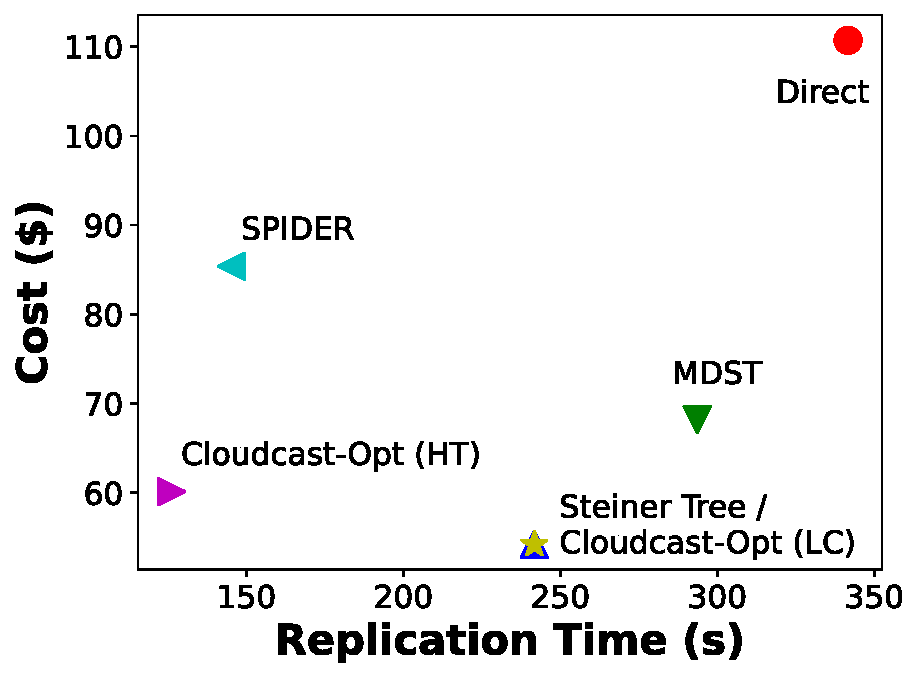
\includegraphics[width=
    0.33\textwidth]{figures/inter_cloud.pdf}
    \caption{Inter-cloud multicast results for different algorithms implemented on \sys{}. The \sys{} replication tree is visualized in Figure \ref{fig:example-topo}.
    % \joey{Figures should have a clear "takeaway" in the caption.  What would you say if presenting this figure in a talk.}
    }
    \label{fig:inter-cloud-1}
\end{figure}





%We run \sys{}-Opt with only two replication time budgets---tight and loose---but we note that \sys{}-Opt is able to find multiple points on the cost-replication time Pareto frontier, as shown in Figure \ref{fig:simulated-baselines}. 
%In fact, \sys{}-Opt can always generate an equivalent cost-minimizing multicast plan to the Steiner Tree, given a loose replication time budget.
%What distinguishes \sys{}-Opt from the Steiner Tree is the ability to trade off cost and replication and also to select the lowest replication time solution among cost-equivalent Steiner Trees. For example, for GCP and Azure intra-cloud transfer, \sys{}-Opt can identify a multicast replication tree of the same cost with $2.5\times$ and $1.6\times$ replication speedup compared to the Steiner Tree.



\subsection{Cloud Provider and P2P Systems}
\label{sec:sys_eval}
We run end-to-end evaluation comparing \sys{} with a commercial baseline (AWS S3 multi-region bucket replication) and P2P systems (BitTorrent and Bullet). 

\subsubsection{AWS S3 Multi-Region bucket replication}
We run an end-to-end comparison between \sys{} and AWS's S3 multi-region bucket replication\cite{aws-replication} for single-provider multicast.
AWS supports adding multiple replication rules to a source bucket to specify automatic replication to one or more replication buckets. 
% NOTE: below line added by Simon
%In comparison, GCP and Azure only support point-to-point transfers and do not provide a data replication product that supports multiple destinations. GCP's multi-region bucket \cite{gcp-multi-region-bucket} does not explicitly transfer to multiple destinations, and it is bounded by geographical regions. 
In the aspect of time control, AWS supports a replication time control with a minimum 15-minute SLO. However, we found that in our experiments, replications typically completed much faster than 15 minutes. Therefore, we use the actual replication time as a point of comparison. 

We compare AWS's replication time and cost to \sys{} with the planner implemented with both direct transfer and the optimizer. 
We transfer an OPT model~\cite{zhang2022opt} with 66 billion parameters ($122$\,GB in total across 9 files) between regions in a single continent\footnote{from \path{aws:ap-east-1} to \path{aws:ap-southeast-2}, \path{aws:ap-south-1}, \path{aws:ap-northeast-3}, \path{aws:ap-northeast-2}, \path{aws:ap-northeast-1}}.
To evaluate AWS replication time and cost, we create buckets with replication rules from a bucket in the source region to buckets in destination regions. 
Once the replication rules are created, we copy data from a bucket in the same region into the source bucket with 16 VMs. After the write completes, we measure the time until the completion of replication into all destination buckets. We calculate the transfer cost according to AWS's pricing page \cite{aws-data-transfer-cost}. We compare AWS multi-region bucket replication to \sys{} implemented with both the direct and optimizer planner and running.  As shown in Figure \ref{fig:aws_comparison}, the direct transfer has the same egress costs as AWS bucket replication, but the VM costs are much less than the service fee charged by AWS for the replication. Overall, \sys{} with the optimizer is able to achieve $2.3\times$ replication speedup and $61.5\%$ cost savings. This is a result of being able to leverage VM parallelism as well as an overlay network that minimizes total egress costs.  

\begin{figure}[t]
    \centering
    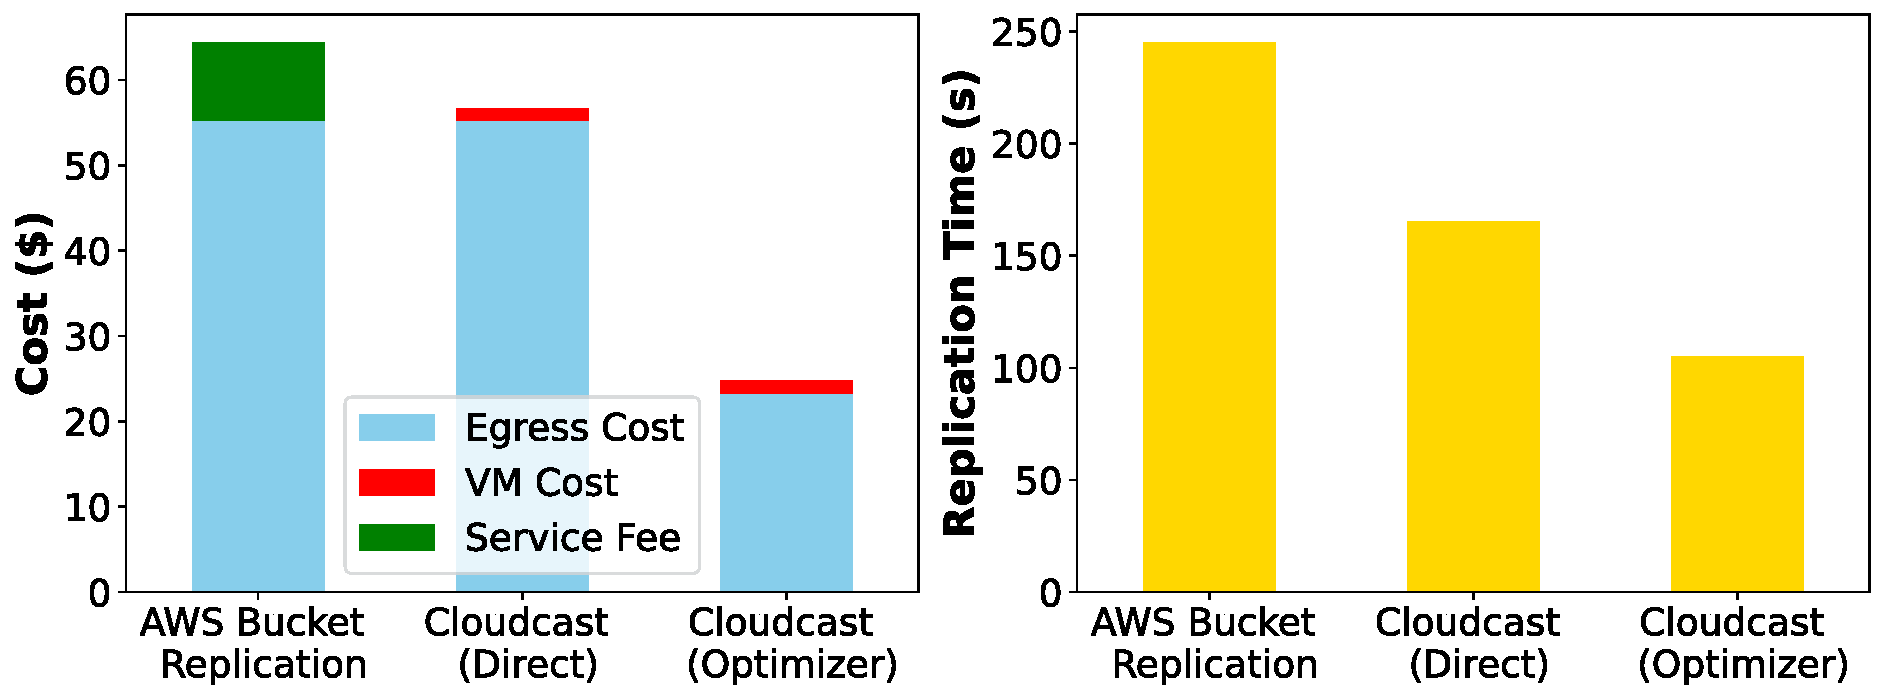
\includegraphics[width=
    \linewidth]{figures/opt_e2e.pdf}
    \caption{\sys{} outperforms AWS S3 Replication Time Control while reducing total transfer costs.} 
    \label{fig:aws_comparison}
\end{figure}

\subsubsection{P2P BitTorrent and Bullet}

We also compare \sys{} against P2P systems like BitTorrent and Bullet. 
%P2P systems are natural choices for transferring large files over multiple destinations. 
We run the same transfer benchmark in Azure in Figure \ref{fig:azure-intra-cloud}, sending 100GB within Azure to 6 destination regions. We host our own BitTorrent tracker and use aria2~\cite{aria2} as a BitTorrent client. Since Bullet's implementation is not available, we evaluate Bullet by implementing Bullet's algorithm inside \sys{}'s planner. The result is shown in Figure \ref{fig:p2p_comparison}: both BitTorrent and Bullet have lower egress costs than direct but higher than \sys{}. BitTorrent is the slowest because most clients cannot utilize the full bandwidth. The clients are built for scenarios like background seeding and transfer off the critical path, rather than for bulk data transfer. Interestingly, without a centralized planner, BitTorrent is able to find a low-cost multicast replication tree by inferring the bandwidth among peers and preferring the data from peers who have the highest throughput. However, it is still significantly more expensive than \sys{}. 
%Peers also communicate with each other by requesting "pieces" and sending "choke" signals. The end result is an all-to-all communication graph that preferred high bandwidth regions like US, Canada, and Europe. 

\begin{figure}[t]
    \centering
     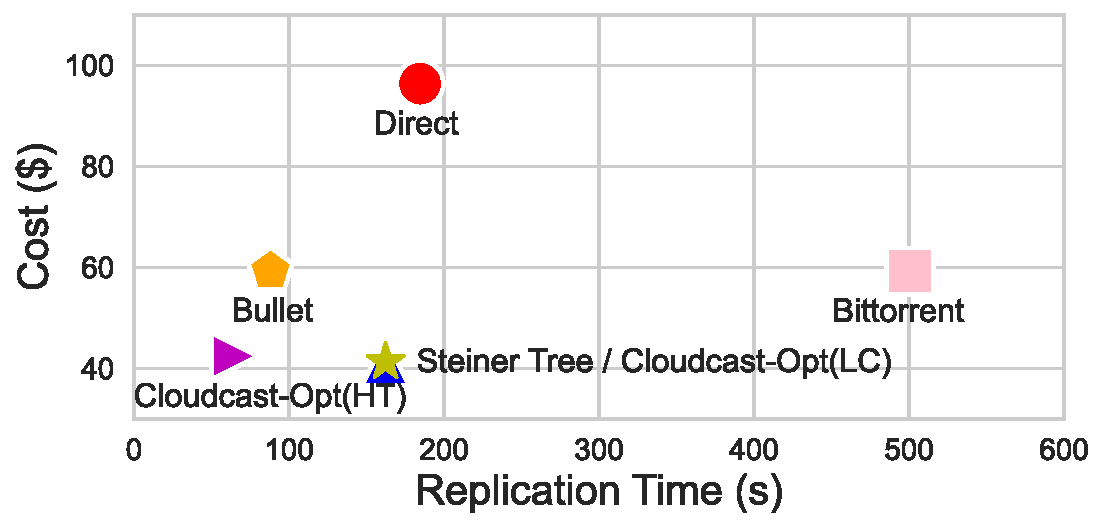
\includegraphics[width=.85\linewidth]{figures/p2p-comparison-all.pdf}
    \caption{Comparison with BitTorrent protocol on the intra-cloud Azure workload in Figure \ref{fig:azure-intra-cloud}. 
    %BitTorrent is cost-conserving as compared to direct transfer. It has the highest runtime because the BitTorrent clients are not designed to efficiently utilize the full available bandwidth.
    }
    \label{fig:p2p_comparison}
\end{figure}

\subsection{Ablations of \sys{}'s Optimizer}
\label{sec:simulated_section}
To understand how our optimizer behaves for different selections of source and destination regions and different target replication times, we run simulated ablations. 
%Due to the high cost of executing many large transfers, in this section, our results evaluate the quality of the plans directly, without execution on the data plane.



\subsubsection{Varying region selection}
\label{random-ablation}
We test the generality of our improvements by randomly selecting source and destination regions for varying numbers of destinations. We show aggregated results over 100 samples for different numbers of destinations in Figure \ref{fig:dest_ablation}. \sys{} is able to improve the runtime and cost of replication consistently across varying numbers of destinations. Cost and throughput improvement increase with more destinations, since more destinations provide a larger optimization space. 

% \begin{figure}[t]
%     \centering
%     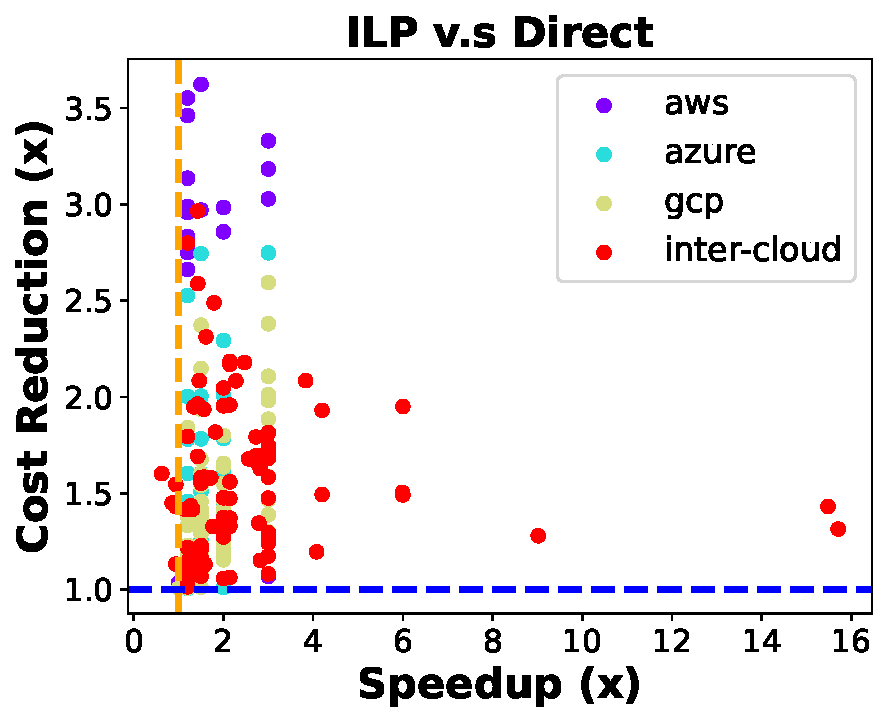
\includegraphics[width=.75\linewidth]{figures/6_dest_100_config.pdf}
%     \caption{\textbf{Simulation: 6 destinations, randomly sampled 100 configurations for Intra-aws/azure/gcp and Inter-cloud transfer)}}
%     \label{fig:random-6-dest}
% \end{figure}


% \begin{figure}[t]
%     \centering
%     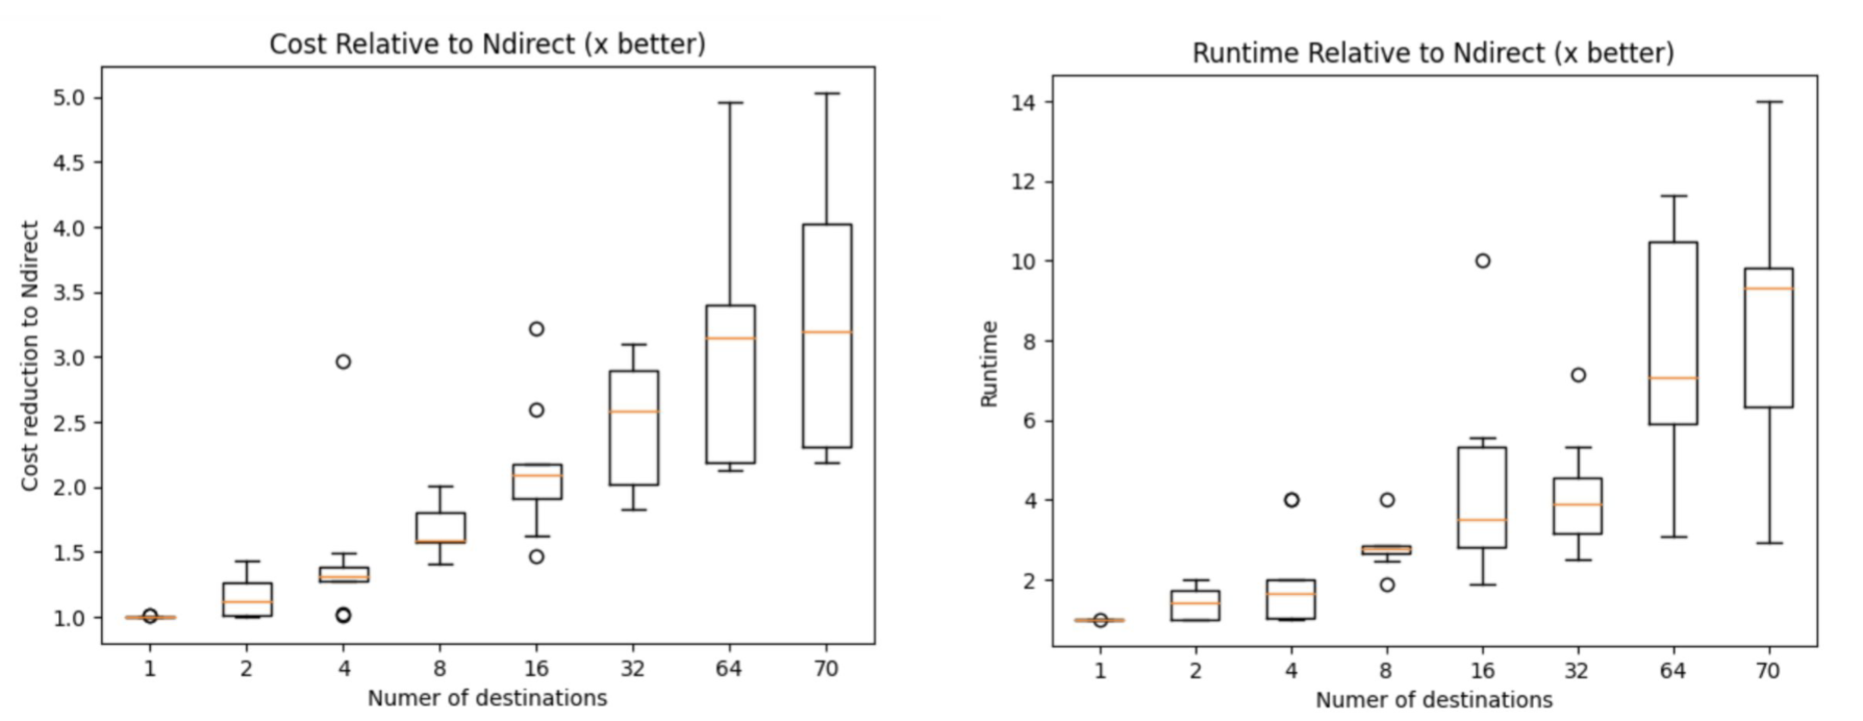
\includegraphics[width=.5\linewidth]{figures/dest_ablation.pdf}
%     \caption{\sys{} optimizer's cost and runtime improvement over direct replication for randomly sampled source and destination regions for varying numbers of destinations.} \label{fig:dest_ablation}
%     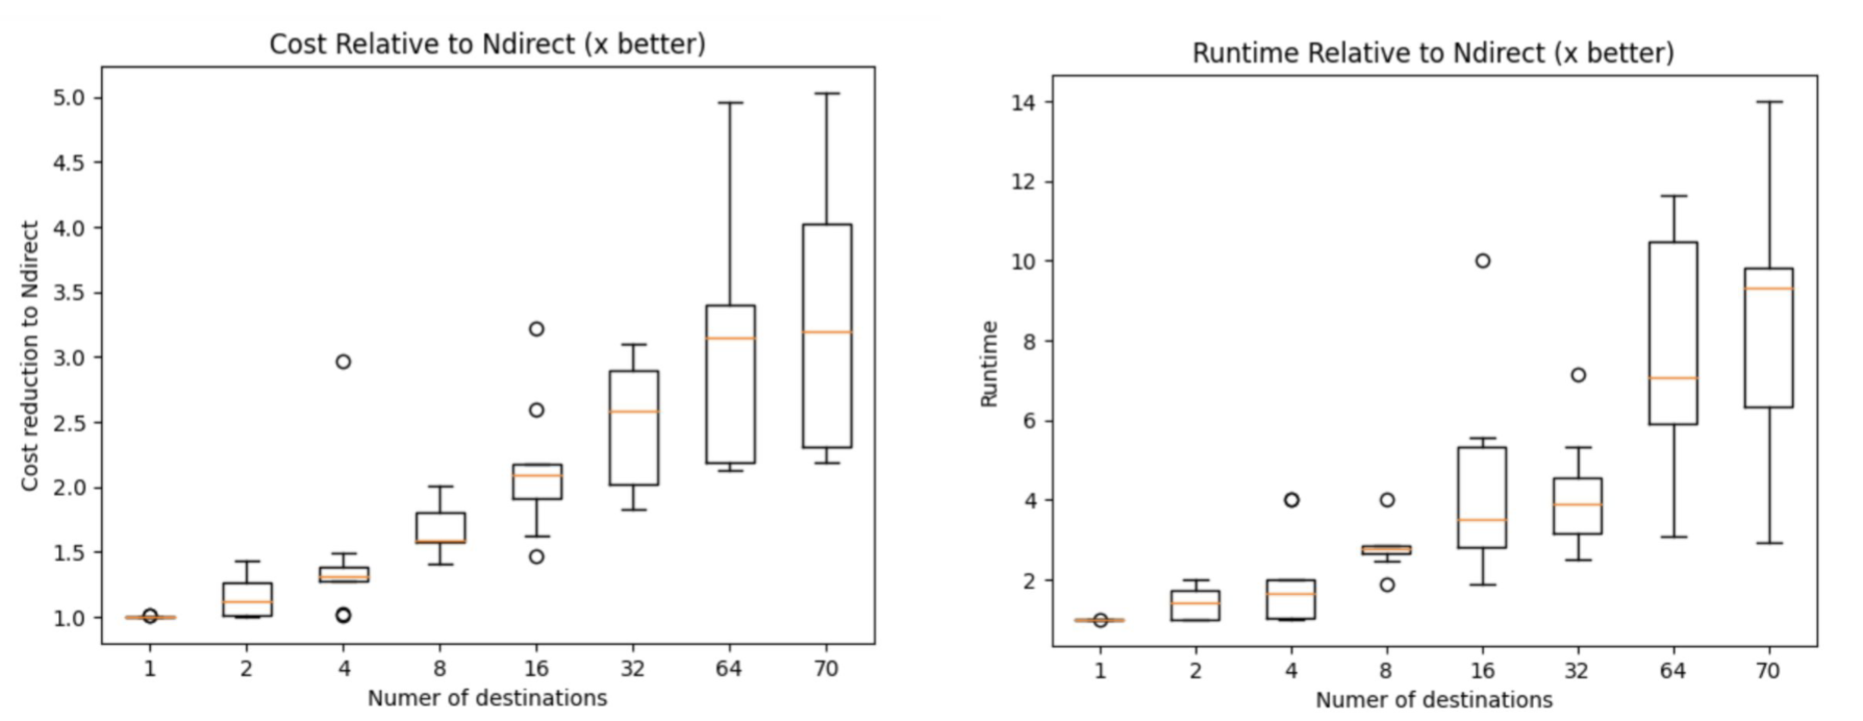
\includegraphics[width=.5\linewidth]{figures/dest_ablation.pdf}
% \end{figure}


\begin{figure}[t]
\centering
\subfloat[][Cost Reduction]{
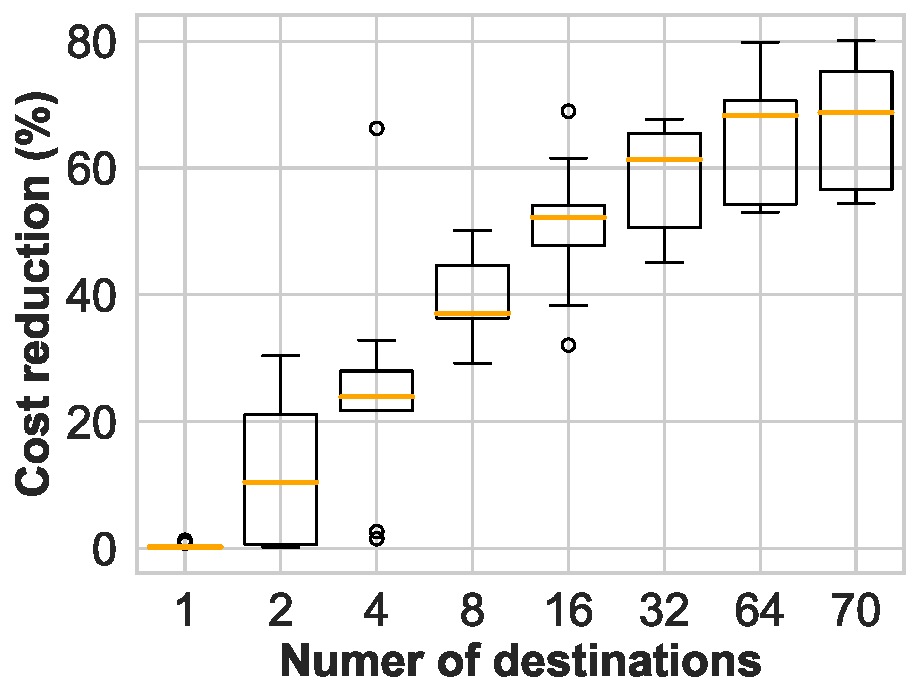
\includegraphics[width=.5\linewidth]{figures/ilp_vary_dest_ndirect_cost_reduction.pdf}\label{fig:dest_ablation1}
} 
\subfloat[][Replication Time Speedup]{
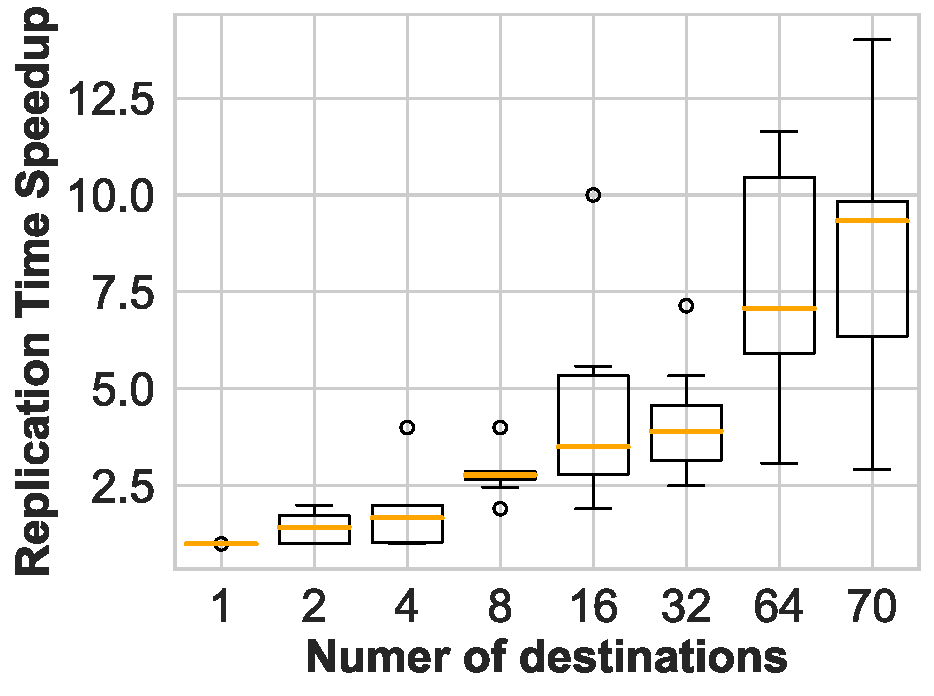
\includegraphics[width=.5\linewidth]{figures/ilp_vary_dest_ndirect_runtime_speedup.pdf}\label{fig:dest_ablation2}
}
\vspace{10pt} % Add extra space above the caption
\caption{\sys{} optimizer's cost and time improvement over direct replication with varying destination numbers.} \label{fig:dest_ablation}
\end{figure}

\subsubsection{Impact of approximations on solutions} 
\label{sss:solution_qual_eval}
% \label{sec:solution_qual_eval}
%As we described in \cref{ss:approximations}, the MILP formulation alone is not practical as a planning algorithm for \sys{} due to solver times that can take hours even for a few destinations. 

%We evaluate how our approximations (node filtering via clustering, hop constraining, and stripe iterative) affect both the solution quality and solver runtime. 

We evaluate how the optimizer with and without approximations scales to larger numbers of destinations in Figure~\ref{fig:solve_time}, by randomly selecting source and destination regions for varying numbers of destination regions. 
%We can see from Figure \ref{fig:solve_time} that 
We find that combining all three approximation mechanisms is necessary to scale the optimizer: using no approximations, or only one approximation, takes several minutes for just 10 destinations while using all approximations together reduces solve time to seconds. 

%For a given number of destinations, we sample a single random combination of source and destination regions, and measure the solver runtime with and without approximations, show in \cref{fig:solve_time}. We terminate the solver at 30 minutes if it cannot solve within that time. We find that we have to terminate the solver with no approximations with only 3 destinations. The stripe-iterative and node-clustering based approximations also can only run up to 7 and 14 destinations respectively and take 100s of seconds for higher numbers of destinations. However, if we combine all approximations together, we can solve for up to 20 destinations in a few seconds. 

\begin{figure}[t]
    \centering
    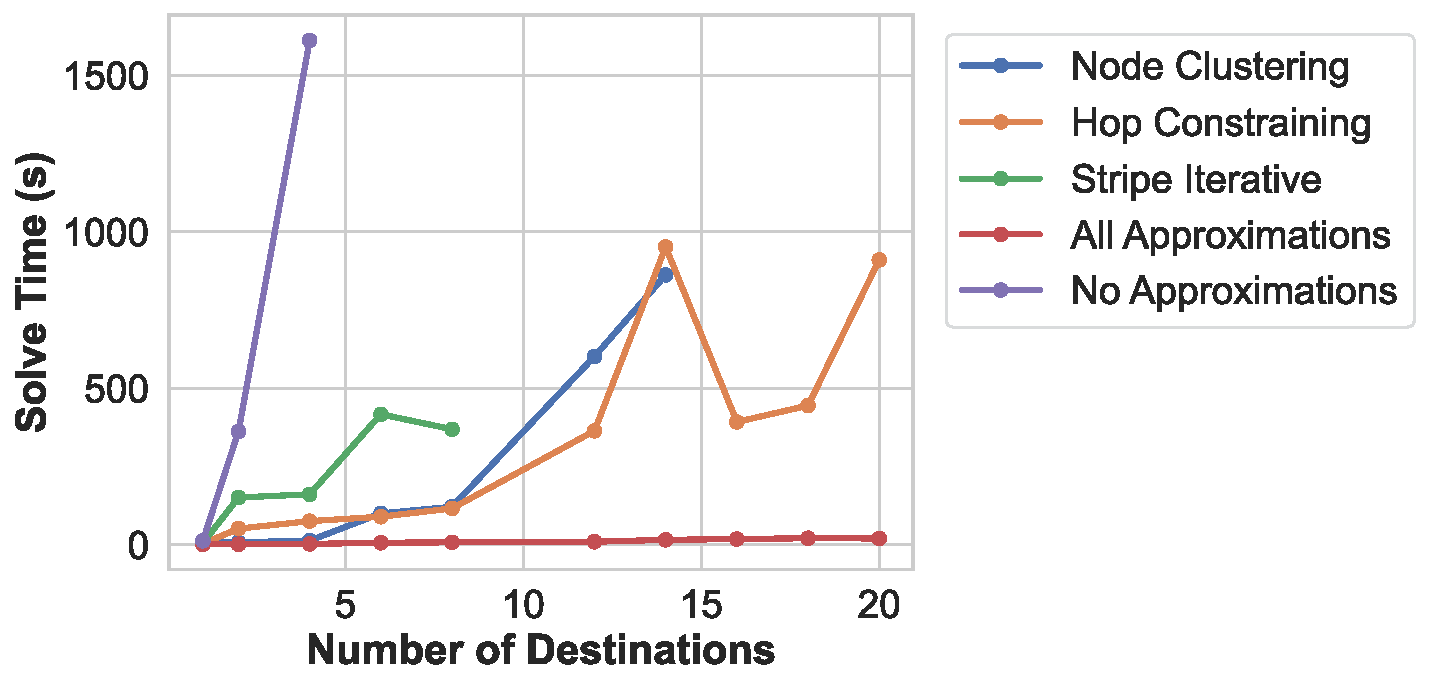
\includegraphics[width=0.9\linewidth]{figures/solve_time_versus_num_dest.pdf}
    \caption{Approximations reduce solver runtime from the cutoff of 30 minutes to seconds for up to 20 destinations.
    % We run the solver with different approximations mechanisms and cutoff measurement at 30 minutes. Without approximations (in purple), the solve time quickly become untenable and cannot reach beyond 4 destinations. With approximations (in red), solve time is within a few seconds even for up to 20 destinations.
    }
    \label{fig:solve_time}
\end{figure}

We also evaluate how approximations affect the quality of the solution using the monetary cost of the solver-generated solution. We randomly sample 100 source/destination combinations for 5 destinations and compute the difference in the solution's monetary cost and replication runtime compared to MILP without approximation in \cref{table:approx-quality}. We find that the difference in cost averages around $1\%$, and estimate the worst-case approximation ratio to be $1.4$. We find that for even just 5 destinations, the approximated solver runs with a geometric-mean speedup of $30.68\times$. %As such, our approximations are reliable and fast.


% \begin{table}[]
% \label{table2}
% \resizebox{\linewidth}{!}{%
% \begin{tabular}{|l|lll|lll|}
% \hline
% \multirow{2}{*}{Approximation} & \multicolumn{3}{l|}{Relative Solve Quality (\%)}               & \multicolumn{3}{l|}{Relative Solve Time Speedup (\times)}        \\ \cline{2-7} 
%                             & \multicolumn{1}{l|}{Min} & \multicolumn{1}{l|}{Max} & Avg & \multicolumn{1}{l|}{Min} & \multicolumn{1}{l|}{Max} & Avg \\ \hline
% \textit{Node Clustering}                        & \multicolumn{1}{l|}{-1.2}    & \multicolumn{1}{l|}{22.7}    &   1.00  & \multicolumn{1}{l|}{-2.5}    & \multicolumn{1}{l|}{50.7}    &   9.04 \\ \hline
% \textit{Hop Constraining}                        & \multicolumn{1}{l|}{-1.2}    & \multicolumn{1}{l|}{44.5}    &   1.01  & \multicolumn{1}{l|}{-0.72}    & \multicolumn{1}{l|}{26.2}    &   5.72 \\ \hline
% \textit{Stripe Iterative}                         & \multicolumn{1}{l|}{-0.4}    & \multicolumn{1}{l|}{0.8}    &   0.02  & \multicolumn{1}{l|}{-0.78}    & \multicolumn{1}{l|}{47.5}    &  7.02 \\ \hline
% \textit{All Approximations}                  & \multicolumn{1}{l|}{-1.7}    & \multicolumn{1}{l|}{\textbf{44.4}}    &  \textbf{1.08}  & \multicolumn{1}{l|}{-4.9}    & \multicolumn{1}{l|}{\textbf{219.1}}   &  \textbf{30.68}   \\ \hline
% \end{tabular}
% }
% \label{fig:approx-quality}
% \caption{Approximation Solve Time and Quality: Compare solution cost and solver runtime with respect to the original MILP for 100 randomly generated 5-destination configurations. Note that since the original MILP itself is an approximation, we are approximating an approximation, so the minimum is sometimes negative (i.e. it is not guaranteed the approximations result in worse solutions).}
% \end{table}
\begin{table}[t]
\centering
\small
\begin{tabular}{lcc}
\toprule
\textbf{Method} &
  \multicolumn{1}{c}{\textbf{Mean error}} &
  \multicolumn{1}{c}{\begin{tabular}[c]{@{}c@{}}\textbf{Solver speedup}\\ \textbf{(geomean)}\end{tabular}} \\ \midrule
\textit{Node Clustering}    & 0.3\% & 9.04$\times$  \\
\textit{Hop Constraining}   & 1.1\% & 5.72$\times$  \\
\textit{Stripe Iterative}   & 0.0\% & 7.02$\times$  \\
\cellcolor{Gray} \textit{All Approximations} & \cellcolor{Gray} 1.1\% & \cellcolor{Gray} 30.68$\times$ \\ \bottomrule
\end{tabular}%
\caption{Solve time and solution quality with approximations.}
\label{table:approx-quality}
\end{table}

%A challenge with making the optimizer practical for real-world use cases is having sufficiently low runtime even for large numbers of destinations and stripes. We reduce the runtime using approximation mechanisms described in \ref{reduce_optimizer_runtime}. We show how approximation mechanisms affect solver quality (in terms of the cost of the solution) and solver runtime in \cref{fig:approx-quality}. 


\subsubsection{Accuracy of replication time model}
\begin{table}[t]
\centering
\small
\begin{tabular}{cc}  
\toprule % Toprule applied here  
  
\textbf{Transfer Size (GB)} & \begin{tabular}[c]{@{}c@{}}\textbf{Prediction error}\end{tabular} \\  
  
\midrule % Midrule applied here  
   
 16 & 16.6\%\\  
 32 & 8.51\%\\  
 64 & 3.31\% \\  
 128 & 1.69\%\\  
\bottomrule % Bottomrule applied here  
\end{tabular}
\caption{Accuracy of the optimizer's predicted throughput.}
\label{table:tp-prediction}
\end{table} 

%Modeling replication throughput is key to ensuring optimizer solutions meet replication time constraints.
We compare optimizer-modeled throughput and real throughput in \cref{table:tp-prediction}.
As transfer size increases, the approximation becomes more accurate.
This is because \sys's optimizer, designed for bulk data replication, makes several simplifying assumptions, such as perfectly pipelined stripes.
Thus, transient inefficiencies during startup and teardown mean smaller transfers may experience lower throughput than the optimizer expects, but for larger, more expensive transfers, modeled throughput closely matches empirical results.

%For smaller transfers, throughput in \sys{} is less than what the optimizer models. However, for larger data transfers, the modeled expected throughput matches the real system throughput.

\subsection{When to Use \sys for Multicast?}
\sys is designed for bulk multicast replication in the cloud, so should only be used with data sizes are sufficiently large. Since \sys relies on creating VMs in the cloud at transfer initiation time, there is a constant overhead from VM startup time. We calculate the transfer size break-even point (i.e. the minimum data size for using \sys{}) for varying providers and VM capacity limits (constraining the throughput for the \sys overlay), shown in Figure~\ref{fig:size_threshold}. We approximate the per-destination replication throughput without \sys as equal to the per-VM egress bandwidth limit, ignoring congestion between source and destination VMs. Azure has a higher break-even point than AWS and GCP due to two effects. First, the VM startup time is the highest of all providers (56 seconds). Second, VMs in Azure are not subjected to egress constraints (5\ Gbps and 7\ Gbps for AWS and GCP, respectively). As a result, the benefits of using \sys's techniques are only realized for larger transfer sizes or larger numbers of destinations. 

\begin{figure}[t]
    \centering
    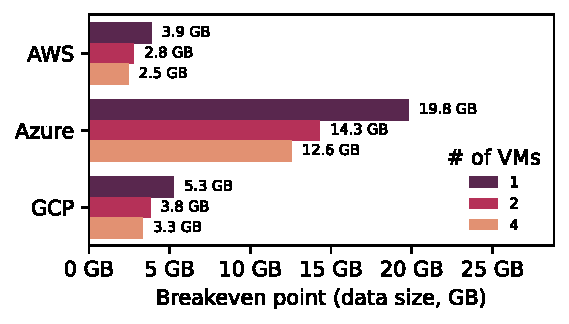
\includegraphics[width=0.7\linewidth]{figures/cloudflare_plot.pdf}
    \caption{Estimated break-even point for a 6-destination replication based on VM startup times ($35$, $56$, and $34$ seconds for AWS, Azure, and GCP, respectively) and VM egress limits. }
    \label{fig:size_threshold}
\end{figure}
%\vincent{what does incumbent mean here?  I would have thought AWS, as the biggest player in the space, is the `incumbent'?}
%\vincent{this is also a bit of a weird eval subsection.  perhaps it should be a section 7 discussion?}

